\chapter{Hydrostatica}
\label{sec:Hydrostatica}
%%%%%%%%%%%%%%%%%%%%%%%%%%%%%%%%%%%%%%%%%%%%%%%%%%%%%%%%%%%%%%%%%%%%%%%%%%%%%%%%%%%%%%%%%
\begin{toepassing}
	\label{koffie}
De chauffeur van een wagen heeft zijn beker koffie in de bekerhouder gezet tijdens het rijden. De beker is cilindervormig met een diameter van 5cm, is gevuld tot op 1cm van de rand en staat horizontaal.
		
Bepaal hoe hard de chauffeur mag remmen of optrekken op een horizontale weg zonder dat hij koffie knoeit.
\end{toepassing}
\begin{antwoord}{\ref{koffie}}
	$a = 4\unit{m/s^2}$
\end{antwoord}
%%%%%%%%%%%%%%%%%%%%%%%%%%%%%%%%%%%%%%%%%%%%%%%%%%%%%%%%%%%%%%%%%%%%%%%%%%%%%%%%%%%%%%%%%
\begin{toepassing}
	\label{rotatiegieten}
Een vloeistof bevindt zich in een ton met diameter 1m die rond zijn as draait met 10 toeren per minuut. In stilstand was de ton gevuld tot 0.2m van de bodem. 
		
Bepaal de vorm van het vloeistof oppervlak na voldoende tijd en de maximale hoogte van de vloeistof.

	\centering
	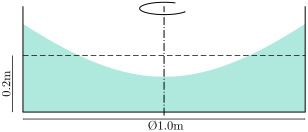
\includegraphics{fig/hydrostatica/rotatiegieten}
\end{toepassing}
\begin{antwoord}{\ref{rotatiegieten}}
	$z = 0.30\unit{m}$ 
\end{antwoord}
%%%%%%%%%%%%%%%%%%%%%%%%%%%%%%%%%%%%%%%%%%%%%%%%%%%%%%%%%%%%%%%%%%%%%%%%%%%%%%%%%%%%%%%%%	
\begin{toepassing}
	\label{u-buis}
Een U-buis gevuld met kwik ($\rho_{Hg}=13600\unit{kg/m^3}$) is aan één zijde verbonden met een leiding waarin olie met een dichtheid van $820\unit{kg/m^3}$ stroomt. De andere zijde is open aan de atmosfeer. In het linker been staat het kwikniveau 0.2m onder de centerlijn van de leiding. Het niveau in het rechterbeen is 0.6m hoger dan het linkerbeen.
		
Bepaal de overdruk in de leiding.

	\centering
	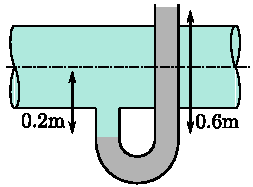
\includegraphics{fig/hydrostatica/u-buis}
\end{toepassing}
\begin{antwoord}{\ref{u-buis}}
	$p = 78.4\unit{kPa}$
\end{antwoord}
%%%%%%%%%%%%%%%%%%%%%%%%%%%%%%%%%%%%%%%%%%%%%%%%%%%%%%%%%%%%%%%%%%%%%%%%%%%%%%%%%%%%%%%%%	
\begin{toepassing}
	\label{u-buizen}
De tanks in onderstaande figuur zijn beide gevuld met lucht. De luchtdruk buiten de tanks is $100\unit{kPa}$. De linker manometer toont een overdruk $p_a=206.9\unit{kPa}$. De 1e U-buis geeft $h_b=1.816\unit{m}$. Beide U-buizen bevatten kwik met een massadichtheid van $13600kg/m^3$.
		
Bepaal het niveau in de 2e U-buis.

	\centering
	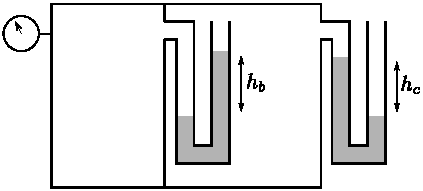
\includegraphics{fig/hydrostatica/u-buizen}
\end{toepassing}
\begin{antwoord}{\ref{u-buizen}}
	$h = 0.295\unit{m}$
\end{antwoord}
%%%%%%%%%%%%%%%%%%%%%%%%%%%%%%%%%%%%%%%%%%%%%%%%%%%%%%%%%%%%%%%%%%%%%%%%%%%%%%%%%%%%%%%%%	
\begin{toepassing}[*]
	\label{u-buis_met_hoogteverschil}
Een leiding met een hoogteverschil heeft twee meetpunten die verbonden zijn met een kwikmanometer ($\rho_{Hg}=13600kg/m^3$) zoals op onderstaande figuur. Het hoogteverschil tussen de twee meetpunten is 0.2m. Het hoogte verschil tussen de kwikniveaus in de manometer is 54mm. Aan het eerste meetpunt is ook een bourdon manometer verbonden die een overdruk van 1.2 bar aangeeft.
		
Bepaal de overdruk in de leiding aan het tweede meetpunt.

	\centering
	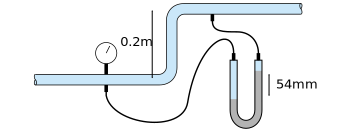
\includegraphics{fig/hydrostatica/u-buis_met_hoogteverschil}
\end{toepassing}
\begin{antwoord}{\ref{u-buis_met_hoogteverschil}}
	$p = 1.1\unit{bar}$
\end{antwoord}
%%%%%%%%%%%%%%%%%%%%%%%%%%%%%%%%%%%%%%%%%%%%%%%%%%%%%%%%%%%%%%%%%%%%%%%%%%%%%%%%%%%%%%%%%	
\begin{toepassing}
	\label{J-buis}
Een J-buis manometer is opgesteld zoals in de figuur om het drukverschil over een regelbare kraan te meten. In de leiding stroomt water met een massadichtheid van $1000kg/m^3$. De manometer is gevuld met kwik met een massadichtheid van $13600kg/m^3$. Bij de huidige stand van de kraan wordt er een hoogteverschil tussen de 2 kwikniveaus gemeten zoals aangegeven op de figuur.
		
Bepaal de drukval over de klep.
		
Bepaal het niveau van het kwik ten opzichte van het huidige onderste niveau wanneer er geen drukval zou zijn. En bepaal de fout die gemaakt wordt wanneer we het hoogteverschil zouden bepalen als het verschil van het hoogste niveau en dit referentie niveau.

	\centering
	\includegraphics{fig/hydrostatica/J-buis}
\end{toepassing}
\begin{antwoord}{\ref{J-buis}}
	$\Delta p = 4032\unit{Pa}$, $\Delta h = 0.317\unit{mm}$,\\ $\Delta p_{\text{fout}} = 40\unit{Pa}$
\end{antwoord}
%%%%%%%%%%%%%%%%%%%%%%%%%%%%%%%%%%%%%%%%%%%%%%%%%%%%%%%%%%%%%%%%%%%%%%%%%%%%%%%%%%%%%%%%%
\begin{toepassing}[*]
	\label{wrijvingskracht}
Een afsluiter van een kanaal is uitgevoerd als een rechthoekig massief paneel. Het paneel heeft een gewicht van 36kN en kan verticaal bewogen worden in geleidingsrails. De wrijvingscoefficient van deze rails ten opzichte van het paneel is 0.2. Het kanaal dat afgesloten wordt is 2m breed en 5m diep.
		
Bepaal de kracht nodig om het paneel naar boven te schuiven.

	\centering
	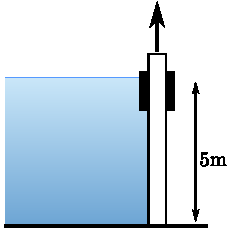
\includegraphics{fig/hydrostatica/wrijvingskracht}
\end{toepassing}
\begin{antwoord}{\ref{wrijvingskracht}}
	$F = 85.1\unit{kN}$
\end{antwoord}
%%%%%%%%%%%%%%%%%%%%%%%%%%%%%%%%%%%%%%%%%%%%%%%%%%%%%%%%%%%%%%%%%%%%%%%%%%%%%%%%%%%%%%%%%
\begin{toepassing}[*]
	\label{stormvloedkering}
Bij hoogwater zijn de waterniveaus aan een stormvloedkering zoals afgebeeld op onderstaande figuur. De kering wordt beschreven door een deel van een cilinder met straal 6m, het middelpunt ligt op 1m van de bodem.
		
Bepaal de horizontale en verticale kracht per lopende meter die door het water wordt uitgeoefend op het oppervlak.

	\centering
	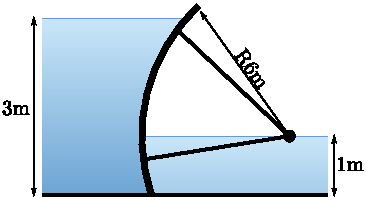
\includegraphics{fig/hydrostatica/stormvloedkering}
\end{toepassing}
\begin{antwoord}{\ref{stormvloedkering}}
	$F_x = 39.2\unit{kN/m}$, $F_y = -0.57\unit{kN/m}$
\end{antwoord}
%%%%%%%%%%%%%%%%%%%%%%%%%%%%%%%%%%%%%%%%%%%%%%%%%%%%%%%%%%%%%%%%%%%%%%%%%%%%%%%%%%%%%%%%%
\begin{toepassing}
	\label{driehoekig_kanaal}
Een driehoekig kanaal met basis 1m en diepte 1m wordt afgesloten door een vlakke plaat.
		
Bepaal de grootte en het aangrijpingspunt van de kracht die op de plaat uitgeoefend wordt.

	\centering
	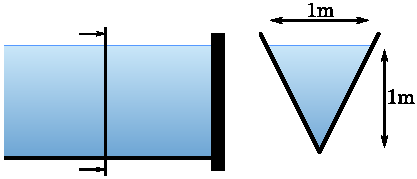
\includegraphics{fig/hydrostatica/driehoekig_kanaal}
\end{toepassing}
\begin{antwoord}{\ref{driehoekig_kanaal}}
	$F = 1.6\unit{kN}$, $z=0.5\unit{m}$ van de bovenzijde
\end{antwoord}
%%%%%%%%%%%%%%%%%%%%%%%%%%%%%%%%%%%%%%%%%%%%%%%%%%%%%%%%%%%%%%%%%%%%%%%%%%%%%%%%%%%%%%%%%
\begin{toepassing}
	\label{sluisklephoek}
Een klep van 6m lengte is scharnierend opgesteld in een kanaal met diepte 4m en breedte 4m. Om de klep in evenwicht te houden wordt er op het uiteinde een constante kracht van 20kN op uitgeoefend loodrecht op het oppervlak van de klep.
		
Bepaal de hoek waaronder de klep zich zal bevinden.

	\centering
	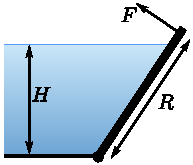
\includegraphics{fig/hydrostatica/sluisklephoek}
\end{toepassing}
\begin{antwoord}{\ref{sluisklephoek}}
	$\alpha = 68\deg$ 
\end{antwoord}	
%%%%%%%%%%%%%%%%%%%%%%%%%%%%%%%%%%%%%%%%%%%%%%%%%%%%%%%%%%%%%%%%%%%%%%%%%%%%%%%%%%%%%%%%%
\begin{toepassing}[*]
	\label{sluisklep}
Een klep aan een sluis heeft een hoogte van 1m. De bovenkant van de klep bevindt zich op 1m onder het wateroppervlak zoals aangegeven op onderstaande figuur.
		
Bepaal de positie van een horizontaal scharnier van de klep zodat deze in evenwicht is in de huidige toestand.

	\centering
	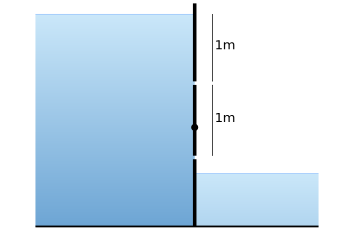
\includegraphics{fig/hydrostatica/sluisklep}
\end{toepassing}
\begin{antwoord}{\ref{sluisklep}}
	$h = 0.44\unit{m}$
\end{antwoord}
%%%%%%%%%%%%%%%%%%%%%%%%%%%%%%%%%%%%%%%%%%%%%%%%%%%%%%%%%%%%%%%%%%%%%%%%%%%%%%%%%%%%%%%%%
\begin{toepassing}[*]
	\label{betonnenligger}
Een betonnen ligger is uitgevoerd zoals op de onderstaande figuur. Deze ligger wordt prefab gegoten met een betonsamenstelling met massadichtheid in vloeibare toestand van 2400kg/m$^3$. De bekisting bestaat uit een bodem paneel, en twee panelen die elk een zijkant vormen. Tijdens het gieten blijft de bovenzijde open liggen.
		
Bepaal de kracht in de horizontale en verticale richting die op de zijpanelen moet worden uitgeoefend bij de productie van een ligger van 10m lang.

	\centering
	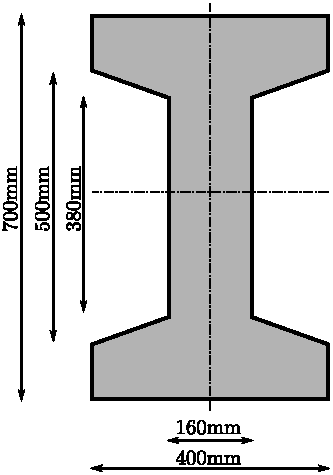
\includegraphics{fig/hydrostatica/betonnenligger}
\end{toepassing}
\begin{antwoord}{\ref{betonnenligger}}
	$F_x = 58.8\unit{kN}$, $F_y = 9.8\unit{kN}$
\end{antwoord}
%%%%%%%%%%%%%%%%%%%%%%%%%%%%%%%%%%%%%%%%%%%%%%%%%%%%%%%%%%%%%%%%%%%%%%%%%%%%%%%%%%%%%%%%%
\begin{toepassing}
	\label{boei}
Een boei heeft de vorm van een bol met diameter 2m. De boei heeft een massa van 2000kg en bevindt zich in zeewater met een dichtheid van $1045\unit{kg/m^3}$. De boei is aan de zeebodem verankerd met een staalkabel met verwaarloosbare massa.
		
Bepaal de kracht in de kabel wanneer de top van de boei 0.5m boven het water uitkomt.

	\centering
	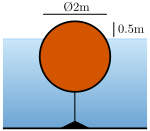
\includegraphics{fig/hydrostatica/boei}
\end{toepassing}
\begin{antwoord}{\ref{boei}}
	$F = 16.6\unit{kN}$ 
\end{antwoord}
%%%%%%%%%%%%%%%%%%%%%%%%%%%%%%%%%%%%%%%%%%%%%%%%%%%%%%%%%%%%%%%%%%%%%%%%%%%%%%%%%%%%%%%%%
\begin{toepassing}
	\label{containerschip}
De dwarsdoorsnede van een containerschip kan benaderd worden zoals op onderstaande figuur. Het schip is 300m lang en heeft een massa van 150000ton. Het massamiddelpunt van het schip bevindt zich in het midden en op een hoogte van 30m boven de kiel. Door ruwe zee is het schip $10\deg$ gekanteld zoals aangegeven op de figuur. De dichtheid van het zeewater wordt geschat op 1045\unit{kg/m^3}
		
Zal het schip kapseizen?
		
	\centering
	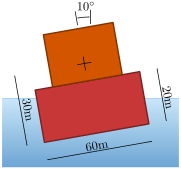
\includegraphics{fig/hydrostatica/containerschip}
\end{toepassing}
\begin{antwoord}{\ref{containerschip}}
	Nee,\\ $x_\text{zwaartepunt}-x_\text{aangrijpingspunt} = 2.16\unit{m}$
\end{antwoord}
	
\section*{Antwoorden}
	\begin{multicols}{2}
		\includecollection{antwoorden}
	\end{multicols}